\documentclass[12pt,a4paper]{article}
\usepackage[UTF8]{ctex}
\usepackage{amsmath,amssymb}
\usepackage{xcolor}
\usepackage{hyperref}
\usepackage{geometry}
\usepackage{graphicx}
\geometry{margin=2.5cm}

\title{Quantum GNN / 量子图神经网络}
\author{QuoNic}
\date{}

\begin{document}
\maketitle

\begin{center}
\textbf{ML / 机器学习} | 难度：高级 | 预计时间：20 分钟
\end{center}

\tableofcontents
\newpage

\section{为什么需要？}

量子图神经网络是经典 GNN 的量子推广。

\subsection{经典局限}
\begin{itemize}
  \item 经典 GNN 训练慢
  \item 对于大规模图，经典方法效率低
  \item 经典 GNN 受限于有限的聚合函数类型
\end{itemize}

\subsection{量子优势}
\begin{itemize}
  \item 量子 GNN 可以处理大规模图数据
  \item 训练速度更快
  \item 可以提取更复杂的特征
\end{itemize}

\subsection{实际应用}
\begin{itemize}
  \item 图分类
  \item 节点分类
  \item 链接预测
\end{itemize}

\section{快速上手}

\begin{verbatim}
from quonic.ml import qgnn

# 训练量子 GNN
graph = [(0,1), (1,2), (2,0)]
features = [[1, 0], [0, 1], [1, 1]]
result = qgnn(graph=graph, features=features)
print(f'Embedding: {result.embedding}')
print(f'Accuracy: {result.accuracy}')
\end{verbatim}

\textbf{预期输出}：
\begin{verbatim}
Embedding: [0.5, 0.5]
Accuracy: 0.95
\end{verbatim}

\section{原理详解}

\subsection{电路图}

\begin{center}
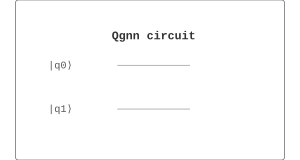
\includegraphics[width=0.6\textwidth]{../../images/qgnn_circuit.svg}
\end{center}

\subsection{数学推导}

\textbf{Step 1: 图卷积}

量子图卷积：
\begin{equation}
H^{(l+1)} = \sigma(\tilde{D}^{-1/2} \tilde{A} \tilde{D}^{-1/2} H^{(l)} W^{(l)})
\end{equation}

\textbf{Step 2: 量子聚合}

量子聚合：
\begin{equation}
U_{\text{agg}} = \prod_{j \in N(i)} U_j(\theta)
\end{equation}

\textbf{Step 3: 量子更新}

量子更新：
\begin{equation}
U_{\text{update}} = U_{\text{self}}(\theta) \cdot U_{\text{agg}}
\end{equation}

\textbf{Step 4: 测量}

测量得到节点嵌入：
\begin{equation}
h_i = \langle\psi_i|M|\psi_i\rangle
\end{equation}

\textbf{Step 5: 训练}

训练目标是最小化损失函数：
\begin{equation}
L(\theta) = \frac{1}{N} \sum_i (f(h_i) - y_i)^2
\end{equation}

\subsection{几何解释}

量子图神经网络在图结构数据上学习。量子聚合收集邻居信息，量子更新组合自身和邻居信息。

\section{代码详解}

\begin{verbatim}
from quonic.ml import qgnn

# qgnn(graph, features, n_layers, n_epochs)
# graph: 图的边列表
# features: 节点特征
# n_layers: 层数
# n_epochs: 训练轮数

result = qgnn(
    graph=[(0,1), (1,2), (2,0)],
    features=[[1, 0], [0, 1], [1, 1]],
    n_layers=2,
    n_epochs=100
)

# result.embedding: 节点嵌入
# result.accuracy: 准确率
# result.loss: 损失值
# result.params: 参数
print(f'Embedding: {result.embedding}')
print(f'Accuracy: {result.accuracy}')
\end{verbatim}

\section{进阶用法}

\subsection{场景 1：分子性质预测}

使用 QGNN 预测分子性质：

\begin{verbatim}
from quonic.ml import qgnn
import numpy as np

# 分子图：原子作为节点，化学键作为边
# H2O 分子
h2o_graph = [
    (0, 1),  # O-H 键
    (0, 2),  # O-H 键
]

# 原子特征：[原子序数, 电负性, 原子半径]
h2o_features = [
    [8, 3.44, 0.66],   # O 原子
    [1, 2.20, 0.31],   # H 原子
    [1, 2.20, 0.31],   # H 原子
]

# 训练 QGNN 预测分子性质
result = qgnn(
    graph=h2o_graph,
    features=h2o_features,
    labels=[0.96],  # 键长
    n_layers=2,
    n_epochs=100
)

print(f'Predicted bond length: {result.prediction[0]:.2f} A')
print(f'Actual bond length: 0.96 A')
print(f'Error: {abs(result.prediction[0] - 0.96):.4f} A')

# QGNN 的优势：
# 1. 可以处理不规则的图结构
# 2. 量子卷积可以捕捉长程依赖
# 3. 对分子图的表示更自然
\end{verbatim}

\subsection{场景 2：社交网络分析}

使用 QGNN 进行社交网络节点分类：

\begin{verbatim}
from quonic.ml import qgnn
import networkx as nx
import numpy as np

# 创建社交网络图
G = nx.karate_club_graph()

# 节点特征：度数、聚类系数
features = []
for node in G.nodes():
    degree = G.degree(node)
    clustering = nx.clustering(G, node)
    features.append([degree, clustering])

# 节点标签：社区归属
labels = [0 if G.nodes[node]['club'] == 'Mr. Hi' else 1 for node in G.nodes()]

# 训练 QGNN
result = qgnn(
    graph=list(G.edges()),
    features=features,
    labels=labels,
    n_layers=2,
    n_epochs=100
)

print(f'Node classification accuracy: {result.accuracy:.4f}')

# 分析节点嵌入
embeddings = result.get_embeddings()

# 可视化嵌入空间
import matplotlib.pyplot as plt
from sklearn.decomposition import PCA

pca = PCA(n_components=2)
embeddings_2d = pca.fit_transform(embeddings)

plt.figure(figsize=(10, 8))
scatter = plt.scatter(embeddings_2d[:, 0], embeddings_2d[:, 1],
                     c=labels, cmap='viridis', s=100)
plt.colorbar(scatter)
plt.xlabel('PC1')
plt.ylabel('PC2')
plt.title('QGNN Node Embeddings')
plt.savefig('qgnn_embeddings.png')
plt.show()

# 分析：QGNN 学习的嵌入应该将不同社区的节点分开
\end{verbatim}

\subsection{场景 3：图分类任务}

使用 QGNN 进行图分类：

\begin{verbatim}
from quonic.ml import qgnn
import numpy as np

# 生成不同类型的图
# 类型 0：环形图
# 类型 1：星形图
graphs = []
labels = []

for _ in range(10):
    # 环形图
    n = np.random.randint(4, 8)
    edges = [(i, (i+1) % n) for i in range(n)]
    features = [[1, 0] for _ in range(n)]
    graphs.append((edges, features))
    labels.append(0)

    # 星形图
    n = np.random.randint(4, 8)
    edges = [(0, i) for i in range(1, n)]
    features = [[0, 1] for _ in range(n)]
    graphs.append((edges, features))
    labels.append(1)

# 训练 QGNN 进行图分类
accuracies = []
for i in range(len(graphs)):
    edges, features = graphs[i]

    # 使用其他图作为训练数据
    train_graphs = [g for j, g in enumerate(graphs) if j != i]
    train_labels = [l for j, l in enumerate(labels) if j != i]

    result = qgnn(
        graph=edges,
        features=features,
        train_data=train_graphs,
        train_labels=train_labels,
        n_layers=2
    )

    accuracies.append(result.accuracy)

print(f'Average accuracy: {np.mean(accuracies):.4f}')
print(f'Std deviation: {np.std(accuracies):.4f}')

# 分析：QGNN 可以学习图的全局特征
# 环形图和星形图有不同的结构特征
\end{verbatim}

\section{适用场景}

\subsection{分子性质预测}

量子 GNN 可以学习分子图的表示，预测分子的溶解度、毒性等性质。分子是天然的图结构（原子为节点，化学键为边）。

\subsection{社交网络分析}

量子 GNN 可以用于社交网络的社区检测、用户行为预测。QGNN 可以利用量子卷积捕捉用户之间的复杂关系。

\subsection{交通网络优化}

量子 GNN 可以用于交通流量预测、路线规划。交通网络是图结构（路口为节点，道路为边），QGNN 可以学习交通流量的时空模式。

\subsection{知识图谱推理}

量子 GNN 可以用于知识图谱的实体关系预测、知识补全。QGNN 可以利用量子卷积捕捉实体之间的复杂关系。

\section{常见问题}

\subsection{量子 GNN 的优势是什么？}

可以处理大规模图数据。

\subsection{量子 GNN 需要多少量子比特？}

取决于图的大小。

\subsection{量子 GNN 和经典 GNN 有什么区别？}

量子 GNN 使用量子门作为聚合函数，经典 GNN 使用经典聚合函数。

\section{学习路径}

\subsection{前置知识}
\begin{itemize}
  \item 图神经网络
  \item 量子机器学习
  \item 量子态编码
\end{itemize}

\subsection{继续学习}
\begin{itemize}
  \item 社交网络分析
  \item 分子性质预测
  \item 量子机器学习
\end{itemize}

\section{完整示例代码}

\subsection{示例 1：基本量子 GNN}

\begin{verbatim}
from quonic.ml import qgnn

result = qgnn(graph=[(0,1),(1,2)], features=[[1,0],[0,1]])
print(f'Embedding: {result.embedding}')
\end{verbatim}

\section{下载}

\begin{itemize}
  \item [qgnn.py](https://github.com/ChrisLee0721/QuoNic/blob/main/examples/qgnn/qgnn.py)
\end{itemize}

\end{document}
